\section{Transition systems for graph rewriting}

\subsection{Graph rewriting}

\begin{definition}[Category of simple graphs]
  We define the category of \emph{simple graphs} where
  \begin{itemize}
  \item objects are graphs: $G = (V,E)$ with $V$ a set of nodes and $E$ a binary symmetric reflexive relation on nodes, representing the edges;
  \item morphisms $h:G_1\to G_2$ are functions on nodes $h_V:V_1\to V_2$ that preserve edges: $(s,t)\in E_1\implies (h_V(s),h_V(t))\in E_2$. We denote $h_E$ the function on edges: $h_E(s,t) = (h_V(s), h_V(t))$.
  \end{itemize}
\end{definition}

A mono is a morphism injective on nodes.

\begin{definition}[Pushout]
  The \emph{pushout} of the span $G_1\leftarrow O\rightarrow G_2$ is the cospan $G_1\rightarrow M\leftarrow G_2$ such that the following diagram commutes
  \[
  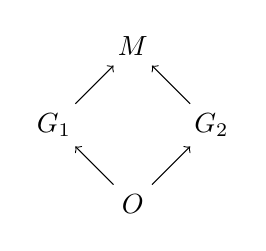
\begin{tikzpicture} %[scale=0.8]
    \node (o) at (0,-1) {\(O\)};
    \node (l1) at (-1,0) {\(G_1\)};
    \node (l2) at (1,0) {\(G_2\)};
    \node (m) at (0,1) {\(M\)};
    \draw [->] (o) --  (l1);
    \draw [->] (o) --  (l2);
    \draw [->] (l1) --  (m);
    \draw [->] (l2) --  (m);
  \end{tikzpicture}
  \]
  and such that for any other cospan $G_1\rightarrow M'\leftarrow G_2$ for which the diagram commutes, there is a unique morphism $M\to M'$:
  \[
  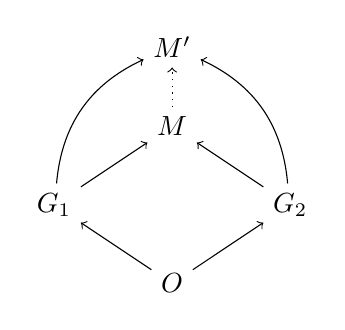
\begin{tikzpicture} %[scale=0.8]
    \node (mp) at (0,2) {\(M'\)};
    \node (o) at (0,-1) {\(O\)};
    \node (l1) at (-1.5,0) {\(G_1\)};
    \node (l2) at (1.5,0) {\(G_2\)};
    \node (m) at (0,1) {\(M\)};
    \draw [->] (o) --  (l1);
    \draw [->] (o) --  (l2);
    \draw [->] (l1) --  (m);
    \draw [->] (l2) --  (m);
    \draw [->] (l1) to [bend left] (mp);
    \draw [->] (l2) to [bend right] (mp);
    \draw [->, dotted] (m) -- (mp);
  \end{tikzpicture}
  \]
\end{definition}

\begin{property}
  \begin{itemize}
  \item The pushout is unique up to isomorphism.
  \item The pushout preserves monos: if $O\to G_i$ is a mono then $G_i\to M$ is also a mono.
  \end{itemize}
\end{property}

\begin{definition}[Double-pushout rewriting]
  Let $p = L\overset{l}{\leftarrow} K \overset{r}{\rightarrow} R$ be a span of injective morphisms, called a \emph{production} or a \emph{rule}. Let $M$ be a graph and $L\lemb M$ be an injective morphism in $M$, called \emph{a matching}.

  The \emph{double pushout transformation} consists in defining the graphs $D'$, called the \emph{context} graph, and the graph $N$ such that in the following diagram:
  \[
  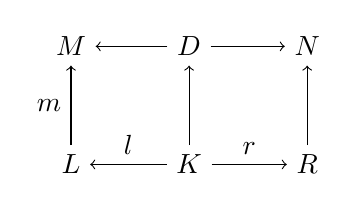
\begin{tikzpicture} %[scale=0.8]
    \node (l) at (-1.5,0) {\(L\)};
    \node (d) at (0,0) {\(K\)};
    \node (r) at (1.5,0) {\(R\)};
    \node (m) at (-1.5,1.5) {\(M\)};
    \node (d') at (0,1.5) {\(D\)};
    \node (n) at (1.5,1.5) {\(N\)};
    \draw [->] (d) -- node [above,midway] {\(l\)} (l);
    \draw [->] (d) -- node [above,midway] {\(r\)} (r);
    \draw [->] (d') -- (m);
    \draw [->] (d') -- (n);
    \draw [->] (l) -- node [left,midway] {\(m\)}  (m);
    \draw [->] (d) -- (d');
    \draw [->] (r) -- (n);
  \end{tikzpicture}
  \]
  the two squares are pushouts.
  We denote $L\action R$ the span $L\overset{l}{\leftarrow} K \overset{r}{\rightarrow} R$. The inverse rule is defined as $p^{-} = R\overset{r}{\leftarrow} K \overset{l}{\rightarrow} L$.
\end{definition}

\begin{property}[Gluing conditions]
  For any graph $G$ let us denote $V_G$ and $E_G$ the corresponding set of nodes and edges, respectively.
  Let $p = L\overset{l}{\leftarrow} K \overset{r}{\rightarrow} R$ be a production and let $L\overset{m}\lemb M$ be a matching in a graph $M$.
  Define the \emph{gluing points} and \emph{dangling points} as the two following sets:
  \begin{align*}
  \text{GP} &= l_V(V_K)\cup l_E(V_E)\\
  \text{DP} &= \{ v\in V_L \big| \exists e\in E_G\setminus m_E(E_L)\text{ s.t. }e=(v,\_)\text{ or }e=(\_, v)\}.
  \end{align*}
  Then DP $\subseteq$ GP iff there exists a unique $D$ such that $L\overset{m}{\rightarrow} M{\leftarrow} D$ is the pushout of the span $ L\overset{l}{\leftarrow} K {\rightarrow} D$.
\end{property}

Henceforth we only consider productions that satisfy the gluing condition.

\begin{remark}
Other graph rewriting techniques exists that allows production with dangling points. However, we are interested in reversible rules, and the DPO approach gives us the inverse of a rule in a straightforward way. We plan to extend the current work to rules with side effect in the future.
\end{remark}

\subsection{Transition systems}

\begin{definition}[Transition systems]
  \label{def:ts_nielsen}
%\cite{NielsenRT92}
  A transition system is a structure $TS = (Q,E,T)$ where $Q$ is a set of states, $E$ is a set of events and $T\subseteq Q\times E\times Q$ is a set of labelled transitions. Let $q_{\text{init}}\in Q$ be a special state, called the \emph{initial} state. Moreover a transition system satisfies the following axioms:
  \begin{itemize}
  \item no redundant events: $\forall e\in E$, $\exists (s,e,s')\in T$;
  \item all states are reachable: $\forall q\in Q$, $\exists q_0,\cdots q_n \in Q$ and $\exists e_o,\cdots e_n\in E$ such that $q_{\text{init}} = q_0$, $q_n =q$ and $(q_i,e_i,q_{i+1}) \in T$;
%  \item no circles:$\forall (s,e,s')\in T$, $s\neq s'$;
%  \item each pair of states connected by a single transition: $\forall (s,e_1,s_1), (s,e_2,s_2)\in T$, $s_1=s_2\implies e_1=e_2$.
  \end{itemize}
\end{definition}

\begin{definition}[TS on graphs]
  A transition system on graphs $TS = (Q,R,E,T)$ consists of
  \begin{itemize}
  \item a set of states $Q$, where each state is a simple graph;
  \item a set of rules or productions, $R$;
  \item a set of events $E$, where each event $e=(p:L\action R,G,m:L\emb G)$ is a triple consisting of a rule $p\in R$, a graph $G$ and a function $m$ that selects one matching $L\emb G$. For an event $e$, we define two functions $\labl(e) = p$ and $m(e) = L\emb G$.
  \item a set of labelled transition $T\subseteq Q\times E\times Q$, where each transition $M \overset{e}{\Rightarrow} N$ is a DPO rewriting step with the production $\labl(e) = p$ and the matching $m(e) = L\emb M$:
    \[
    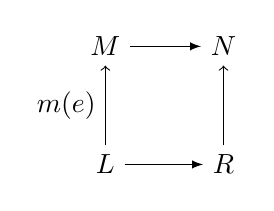
\begin{tikzpicture} %[scale=0.8]
      \node (l) at (-1.5,0) {\(L\)};
      \node (r) at (0,0) {\(R\)};
      \node (m) at (-1.5,1.5) {\(M\)};
      \node (n) at (0,1.5) {\(N\)};
      \draw [->] (l) -- node [left,midway] {\(m(e)\)}  (m);
      \draw [>=latex, ->] (l) -- (r);
      \draw [>=latex, ->] (m) -- (n);
      \draw [->] (r) -- (n);
    \end{tikzpicture}
    \]
    We sometimes write $M\overset{m(e),\labl(e)}{\Rightarrow} N$.
  \end{itemize}
  Moreover $TS$ satisfy the axioms of~\autoref{def:ts_nielsen}.
\end{definition}

\begin{definition}[Independence relation~\cite{AlgebraicGR}]
  \label{def:indep}
  $~$
  \begin{description}
  \item[sequential independence]
    Let $M\overset{m_1,p_1}{\Rightarrow} M_1$ and $M_1\overset{m_2,p_2}{\Rightarrow} M_2$ be two transitions.
    $(p_1,M,m_1) \Diamond_{\text{seq}} (p_2,M_1,m_2)$ iff there exists the morphism $i:R_1\to D_2$ such that $f_2\circ i= m_2$ and there exists the morphism $j:L_2\to D_1$ such that $g_1\circ j= m_1$:
    \[
    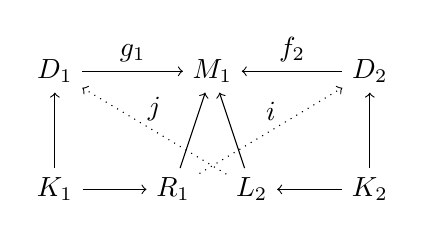
\begin{tikzpicture} %[scale=0.8]
    \node (r1) at (1.5,0) {\(R_1\)};
    \node (m1) at (2,1.5) {\(M_1\)};
    \node (l2) at (2.5,0) {\(L_2\)};
    \node (d1) at (0,1.5) {\(D_1\)};
    \node (k1) at (0,0) {\(K_1\)};
    \node (d2) at (4,1.5) {\(D_2\)};
    \node (k2) at (4,0) {\(K_2\)};
    \draw [->] (k1) -- (r1);
    \draw [->] (k2) -- (l2);
    \draw [->] (k1) -- (d1);
    \draw [->] (k2) -- (d2);
    \draw [->] (d1) -- node [above,midway] {\(g_1\)} (m1);
    \draw [->] (d2) -- node [above,midway] {\(f_2\)} (m1);
    \draw [->] (l2) -- (m1);
    \draw [->] (r1) -- (m1);
    \draw [dotted,->] (r1) -- node [above,midway] {\(i\)} (d2);
    \draw [dotted,->] (l2) -- node [above,midway] {\(j\)} (d1);
    \end{tikzpicture}
    \]
  \item[parallel independence]
    Let $M\overset{m_1,p_1}{\Rightarrow} M_1$ and $M\overset{m_2,p_2}{\Rightarrow} M_2$ be two transitions.
    $(p_1,M,m_1) \Diamond_{\text{par}} (p_2,M,m_2)$ iff there exists the morphism $i:L_1\to D_2$ such that $f_2\circ i= m_2$ and there exists the morphism $j:L_2\to D_1$ such that $f_1\circ j= m_1$:
    \[
    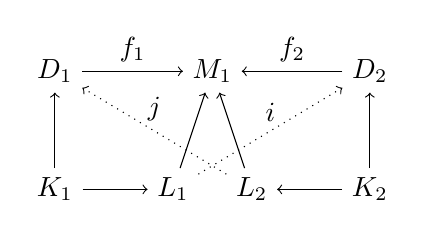
\begin{tikzpicture} %[scale=0.8]
    \node (r1) at (1.5,0) {\(L_1\)};
    \node (m1) at (2,1.5) {\(M_1\)};
    \node (l2) at (2.5,0) {\(L_2\)};
    \node (d1) at (0,1.5) {\(D_1\)};
    \node (k1) at (0,0) {\(K_1\)};
    \node (d2) at (4,1.5) {\(D_2\)};
    \node (k2) at (4,0) {\(K_2\)};
    \draw [->] (k1) -- (r1);
    \draw [->] (k2) -- (l2);
    \draw [->] (k1) -- (d1);
    \draw [->] (k2) -- (d2);
    \draw [->] (d1) -- node [above,midway] {\(f_1\)} (m1);
    \draw [->] (d2) -- node [above,midway] {\(f_2\)} (m1);
    \draw [->] (l2) -- (m1);
    \draw [->] (r1) -- (m1);
    \draw [dotted,->] (r1) -- node [above,midway] {\(i\)} (d2);
    \draw [dotted,->] (l2) -- node [above,midway] {\(j\)} (d1);
    \end{tikzpicture}
    \]
  \end{description}

%We call such a TS an \emph{asynchronous} transition system~\cite{Mukund93}.
\end{definition}

\begin{lemma}[Local Church Rosser Theorem for GT systems\cite{AlgebraicGR}]
  \label{church_rosser}
  If two transitions $M\overset{m_1,p_1}{\Rightarrow} M_1$ and $M_1\overset{m_2,p_2}{\Rightarrow} M_2$ are sequentially independent, there exists $M'\in Q$ and two transitions $M\overset{m_2',p_2}{\Rightarrow} M'$ and $M'\overset{m_1',p_1}{\Rightarrow} M_2$. If two transitions $M\overset{m_1,p_1}{\Rightarrow} M_1$ and $M\overset{m_2,p_2}{\Rightarrow} M_2$ are parallel independent, then there exists $M'\in Q$ and two transitions $M_1\overset{m_2',p_2}{\Rightarrow} M'$ and $M_2\overset{m_1',p_1}{\Rightarrow} M'$.
\end{lemma}

We equip a graph transition system $(Q,R,E,T)$ with an irreflexive, symmetric relation on events $\Diamond\subseteq E\times E$, called independence, such that $e_1\Diamond e_1$ iff $e_1\Diamond_{\text{seq}} e_1$ or $e_1\Diamond_{\text{par}} e_1$.

\begin{definition}[Sequential dependence]
  \label{def:seq_dep}
  Transitions $M\overset{m_1,p_1}{\Rightarrow} M_1$ and $M_1\overset{m_2,p_2}{\Rightarrow} M_2$ are sequential dependent if there exists no morphism  $j:L_2\to D_1$ such that $f_1\circ j= m_1$. We denote $(p_1,M,m_1) < (p_2,M_1,m_2)$.
\end{definition}

\autoref{def:seq_dep} implies that if $M\overset{m_1,p_1}{\Rightarrow} M_1$ and $M_1\overset{m_2,p_2}{\Rightarrow} M_2$ are sequential dependent then ther is no graph $M'\in Q$ such that $M\overset{m_2',p_2}{\Rightarrow} M'$ and $M'\overset{m_1',p_1}{\Rightarrow} M_2$ and such that $(p_1,M,m_1)\Diamond_{\text{par}}(p_2,M,m_2')$.

\begin{definition}[Parallel dependence]
  \label{def:inhibition}
  A transition $M\overset{m_1,p_1}{\Rightarrow} M_1$ inhibits another transition $M\overset{m_2,p_2}{\Rightarrow} M_2$ if there is no morphisms $j:L_2\to D_1$ such that $f_1\circ j= m_1$. We denote $(p_1,M,m_1) \dashv (p_2,M_1,m_2)$.
  The two transitions are parallel dependent if they are inhibiting each other.

%  Define $\dashv\subseteq E \times E$ a relation on events such that whenever $e_1\dashv e_2$ there exists two transitions $M\overset{m_1,p_1}{\Rightarrow} M_1$ and $M\overset{m_2,p_2}{\Rightarrow} M_2$ for which %i.e. $m_{e_2}(M_1) = \emptyset$, where $\labl(e_1)=p_1$, $m_{e_1}(M) = m_1$ and $\labl(e_2)=p_2$, $m_{e_2}(M) = m_2$.
\end{definition}

From~\autoref{def:inhibition} we have that if $(p_1,M,m_1) \dashv (p_2,M_1,m_2)$ then there is no graph $M'\in Q$ such that $M_1\overset{m_2',p_2}{\Rightarrow} M'$ and such that $(p_1,M,m_1)\Diamond_{\text{seq}}(p_2,M_1,m_2')$.

\begin{lemma}
  If two transitions $M\overset{m_1,p_1}{\Rightarrow} M_1$ and $M_1\overset{m_2,p_2}{\Rightarrow} M_2$ are not sequentially independent, then either $(p_1,M,m_1) < (p_2,M_1,m_2)$ or $(p_2,M,m_2)\dashv(p_1,M,m_1)$ (or both).
\end{lemma}
\begin{proof}
  If $M\overset{m_1,p_1}{\Rightarrow} M_1$ and $M_1\overset{m_2,p_2}{\Rightarrow} M_2$ are not sequentially independent, from~\autoref{def:indep}, it follows that either (i) there is no morphism $j:L_2\to D_1$ such that $g_1\circ j= m_1$ and then $(p_1,M,m_1) < (p_2,M_1,m_2)$ or (ii)
there is no morphism $i:R_1\to D_2$ such that $f_2\circ i= m_2$. Suppose for the latter case, that there is $j:L_2\to D_1$ such that $g_1\circ j= m_1$. It implies, from~\autoref{church_rosser} that there exists $M'\in Q$ and $M\overset{m_2',p_2}{\Rightarrow} M'$ and that $(p_1,M,m_1)$ is not parallel independent of $(p_2,M,m_2')$. From the definition of parallel independence the only possibility is that there is no morphism $i:L_1\to D_2$ such that $f_2\circ i= m_2$. \autoref{def:inhibition} implies then that $(p_2,M,m_2)\dashv(p_1,M,m_1)$.
\end{proof}

\begin{lemma}
  If two transitions $M\overset{m_1,p_1}{\Rightarrow} M_1$ and $M\overset{m_2,p_2}{\Rightarrow} M_2$ are not parallel independent then either $(p_1,M,m_1)\dashv(p_2,M,m_2)$ or $(p_2,M,m_2)\dashv(p_1,M,m_1)$ (or both).
\end{lemma}
The proof is similar to the one above.
